\chapter{Radio Interferometry}

Since this work analyzes mostly data from radio observations, in particular using interferometer array, in this chapter we briefly review some basic concepts of radio interferometric observations. We also describe some basic properties of the ALMA radio telescope.  

The angular resolution ($\theta_{\text{res}}$) of single dish radio telescope is given by 
\begin{equation}
\theta_{\text{res}} = 1.22\ \frac{\lambda}{D},
\label{eq:thetares}
\end{equation}
where $\lambda$ is the wavelength and $D$ is the diameter of the telescope. The intensity distribution of an incoming signal can be calculated by using a Bessel's function, so that the approximation of the first Bessel's function becoming zero leads to the numerical factor of 1.22. 

For the same diameter size, observations in longer wavelength (radio) result in a smaller angular resolution. To improve the angular resolution for an observation at a given wavelength, the diameter of the telescope has to be increased. Fortunately, in radio wavelenths, this can be done by synchronization of multiple radio telescopes called radio interferometry techniques. The resolution of the system is comparable to the distance of the longest baseline, i.e., the farthest distance between two telescopes.

\section{Aperture Synthesis}

The simplest array of telescopes consists of two identical antennas, hence the concept of radio interferometry can be explained with much simplification by the so called two-element interferometer (\autoref{fig:twoline}). The following explanations and descriptions are adapted from \cite{burke2014} and ALMA Technical Handbook \citep{almatech2016}.

\begin{figure}[!ht]
\centering
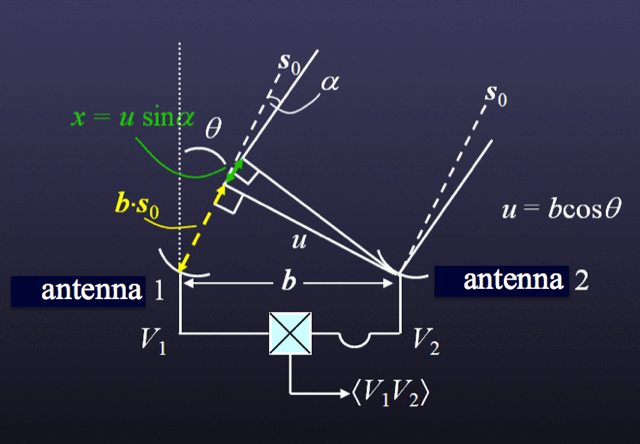
\includegraphics[width=0.7\textwidth]{fig/baseline.png}
\caption{Two-element interferometer, consists of two antennas. Ilustration from ALMA Technical Handbook (\citeyear{almatech2016}).}
\label{fig:twoline}
\end{figure}

The power received by one single telescope/element is given by
\begin{equation}
P = \int_{0}^{\infty} A_{\text{eff}}(\nu) S(\nu) d \nu,
\end{equation}
where $S(\nu)$ is the flux density of the source, given by its brightness distribution integrated over the solid angle, and $A_{\text{eff}}(\nu)$ is the effective area of the dish. In the radio interferometry, this power is converted into voltage. Since the power is proportional to the square of voltage, to recover the flux receive from the source, we need to multiply the voltage response from each antenna (that is, auto-correlation and cross correlation).

\autoref{fig:twoline} shows a schematic diagram of a two-element interferometer separated by a distance $L$. We can measure this distance in units of the observing wavelength ($\lambda$), $b = L/\lambda$, usually called baseline. Both antennas observe a common position $s_0$ located at an angle $\theta$ from the meridian. The projected separation of the two antennas towards $s_0$ from the perspective of the source is $u = b \cos \theta$. The signal arrives at the first antenna delayed by the geometrical delay $\tau_g = \frac{b \cdot s_0}{c}$. To compensate for the geometrical delay, an artificial delay can be inserted into the signal path of antenna 2 (e.g., electronically) so that the signals from both antennas arrive at the correlator with the same phase.

Moving slightly off-axis, we can describe a small angle from the axis as $\alpha$, and its 1-D sky position as $l = \sin \alpha$. At angle $\alpha$, an off-axis signal reaching antenna 1 will have to travel a slightly longer path than an off-axis signal reaching antenna 2, even with the geometrical delay introduced to compensate for an on-axis signal. This extra path length is $x = u \sin \alpha = ul$. It turs out that the extra path lengths result in phase differences with $\alpha$ that can be characterized where the voltage response of antenna 2, $V_2$, can be written in terms of the product of the voltage response of antenna 1, $V_1$, and a phase delay factor sinusoidally varying as a function of angle, that is,
\begin{equation}
V_2 = V_1 e^{2 \pi i u l}
\end{equation}

In 2-D case, we can define similar angle in orthogonal direction, and the equation becomes
\begin{equation}
V_2 = V_1 e^{2\pi i (ul + vm)},
\end{equation}
where $u$ and $v$ is called specific spatial frequency components of the sinusoid in the East-West and North-South directions, respectively, and these are the projected lengths of the antenna separations measured in units of the wavelength at the time of observation. In addition, we identify $l$ and $m$ as direction cosines relative to a reference position in the E-W and N-S directions, respectively. The on-axis position $s_0$ has $l = 0$ and $m = 0$ and is called the phase center.

The correlator acts as a multiplying and time-averaging device for the incoming signals from antennas 1 and 2,
$$\left\langle V_1 V_2 \right\rangle = \left\langle \int\int V_1 (l,m) dl dm  \int\int V_2 (l,m) dl dm \right\rangle$$
Under the assumption that signals emanating from different parts of the sky are incoherent, the time averages of the correlation of those signals will be zero. Thus, the product of the integrals can be simplified into the form 
\begin{eqnarray}
\left\langle V_1 V_2 \right\rangle &=& \left\langle \int\int V_1 (l,m) V_2 (l,m) dl dm \right\rangle \\
&=& \int\int \left\langle V_1 (l,m)^2 \right\rangle e^{2 \pi i (ul + vm)} dl dm \\
&=& \int\int I(l, m) e^{2 \pi i (ul + vm)} dl dm 
\end{eqnarray}
where $I(l, m)$ is the intensity distribution on the sky. The correlator therefore measures a quantity known as the ``complex visibility'', $\mathcal{V}$, which is formally the Fourier transform of the intensity distribution on the sky:
\begin{equation}
\mathcal{V}(u,v) = \int \int I(l, m) e^{2 \pi i (ul + vm)} dl dm = A e^{i\phi}
\end{equation}
$\mathcal{V}$ is a complex number, and can be described by an amplitude $A$ and a phase $\phi$. The amplitude and phase contain information about the source brightness and its location relative to the phase center, respectively, at spatial frequencies $u$ and $v$.

The relationship between the sky brightness distribution and the complex visibility distribution is governed by the \textit{van Cittert-Zernike theorem} which says that ``Complex visibility is the Fourier transform of the sky brightness distribution in the image plane''. It is the basis of the aperture synthesis.

It follows that ``the sky brightness distribution is in turn the inverse Fourier transform of the complex visibility distribution in the visibility plane'' or $uv$-\textit{plane}.
\begin{equation*}
I(l, m) = \int \int \mathcal{V}(u, v) e^{-2 \pi i (ul + vm)} du dv 
\end{equation*}

Theoretically, by measuring all of the \textit{complex visibilities}, we can reconstruct the true sky brightness. However, in reality not all of $uv$-plane can be sampled because of the limit on the number of the antenna or baseline combination. 

To reconstruct the true sky brightness we need to use \textit{deconvolution} technique, usually called  `CLEAN'ing procedure. Moreover, due to incompleteness of spatial frequency sampled from observation, we need to choose the configuration of the antenna array that can recover at maximum the features or details seen on the target object. To recover small features, we need more sparse array configuration. On the other hand, we need more compact configuration to recover large features of the target. 


\section{Atacama Large Millimeter/submillimeter Array (ALMA)}

The Atacama Large Millimeter/submillimeter Array (ALMA) is a new facility of radio interferometer array consisting of 66 
antennas (that is, 54 antennas of the 12-m diameter and 12 antennas of the 7-m diameter) that can be arranged in a series of 
different configurations, covering a baseline of a few meters up to 18 km. The ALMA 
antennas are located on the Chajnantor Plateau, Chile (lat. = -23.02917$^{\circ}$, long. = -67.754649$^{\circ}$)
at the altitude of 5000 m. Therefore, this site represents one of the driest place in the world (see \autoref{fig:ALMAtransmission}) 
and is very suitable to host radio telescopes that can
operate over a broad range of observing frequencies in the millimeter and submillimeter range. ALMA Early Science 
Operations started with Cycle 0 in September 2011 (with less than 20 antennas) and the official inauguration took place in March 2013. 
Long baseline campaigns have been started in Cycle 3 and succesfully yielded many remarkable results. After subsequent
development, ALMA presently works in Cycle 4 with more advanced capability. 

\begin{figure}[!ht]
\centering
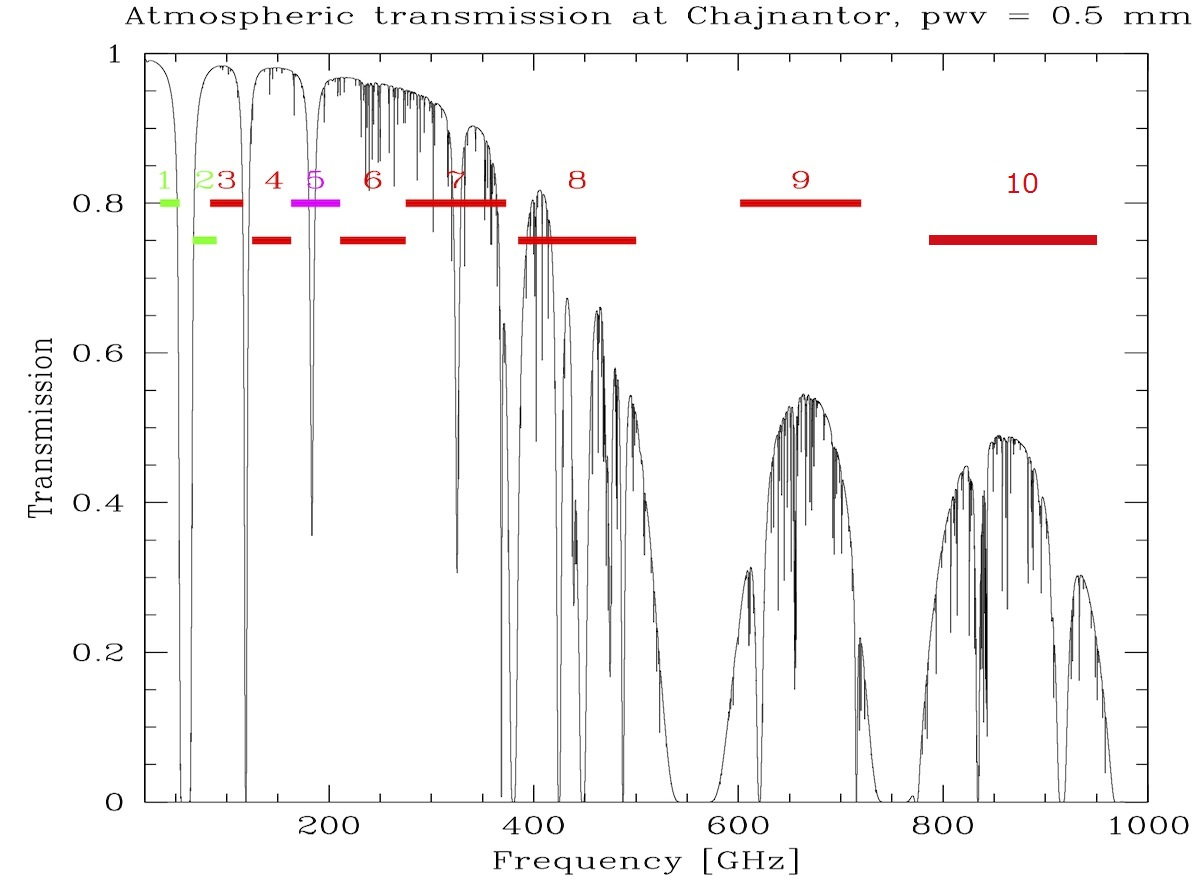
\includegraphics[width=0.99\textwidth]{fig/transmission.png}
\caption[ALMA receiver bands for Cycle 4 (2017)]{The ten ALMA receiver bands. Receiver bands for Cycle 4 (2017) are shown in red superimposed on a zenith atmospheric transparency plot for 0.5 mm of PWV.}
\label{fig:ALMAtransmission}
\end{figure}

\begin{table}[!ht]
\centering
\caption[ALMA receivers characteristics.]{ALMA receivers characteristics. Band 1 and 2 are still in the development process, Band 4, 9, 10 are only operated recently, Band 5 not used for science. Configuration, SSB: single sideband; 2SB: both sidebands detected separately; DSB: double sideband.}
\label{tab:ALMAreceiver}
\begin{tabular}{ccccc}
\hline
Band   & Frequency Range & Wavelength & Instantaneous   & Config \\
Number & (GHz)           & (mm)       & Bandwidth (GHz) &               \\
\hline
1      & 31.3 -- 45.0     & 6.7 -- 9.6  & 1 $\times$ 8           & SSB           \\
2      & 67 -- 90         & 3.3 -- 4.5  & 1 $\times$ 8           & SSB           \\
3      & 84 -- 116        & 2.6 -- 3.6  & 2 $\times$ 4           & 2SB           \\
4      & 125 -- 163       & 1.8 -- 2.4  & 2 $\times$ 4           & 2SB           \\
5      & 163 -- 211       & 1.4 -- 1.8  & 2 $\times$ 4           & 2SB           \\
6      & 211 -- 275       & 1.1 -- 1.4  & 2 $\times$ 5.5         & 2SB           \\
7      & 275 -- 373       & 0.8 -- 1.1  & 2 $\times$ 4           & 2SB           \\
8      & 385 -- 500       & 0.6 -- 0.8  & 2 $\times$ 4           & 2SB           \\
9      & 602 -- 720       & 0.4 -- 0.5  & 2 $\times$ 8           & DSB           \\
10     & 787 -- 950       & 0.3 -- 0.4  & 2 $\times$ 8           & DSB   \\
\hline
\end{tabular}
\end{table}

The ALMA front end can accommodate up to 10 receiver bands (\autoref{tab:ALMAreceiver}) covering most of the 
wavelength range from 10 to 0.3 mm (30 \--- 950 GHz). Each receiver band is designed to cover atmospheric transmission 
windows in this range of frequency (\autoref{tab:ALMAreceiver}). The angular resolution can reach up to $0.02''$ 
(for example, at $\lambda = 1$  mm and 10 km baseline), with the baseline range from 15 m to 18 km. \autoref{fig:ALMAtransmission} shows 
the atmospheric transmission in ALMA site with a typical precipitable water vapour (PWV) of 0.5 mm 
together with the coverage of ALMA observing bands. As previously mentioned, 
the receiver bands that have strong interest in this work are Bands 3, 6, 7, and 9. We can `see' the synchrotron radiation in Band 3, on the other hand Band 6, 7, and 9 usually used to `see' the dust emission from the galaxy. 


%\subsubsection*{ALMA Cycle and Data}
%\begin{itemize}
%\item Cycle 0
%\item Cycle 1
%\item Cycle 2
%\item Cycle 3
%\end{itemize}

\cleardoublepage
